
\documentclass[handout,12pt,dvipsnames,t]{beamer}
\setbeamertemplate{footline}[frame number]
%\usepackage{pgfpages}
%\pgfpagesuselayout{4 on 1}[a4paper,border shrink=5mm,landscape]

\title{Statistical Practice in Epidemiology 2018 \newline }
\subtitle{Survival analysis with competing risks} % \\[10mm]
\author{Janne Pitk\"aniemi (EL) }
\date{}
\usepackage{Sweave}
\begin{document}
\Sconcordance{concordance:Survival_competing_risk.tex:Survival_competing_risk.Rnw:%
1 7 1 1 0 804 1}


\maketitle


\begin{frame}[fragile]
\frametitle{Points to be covered}

\begin{itemize}
\item[1.] Survival or time to event data \& censoring.
 \medskip
 \item[2.] 
 Competing risks: event-specific cumulative incidences \& hazards.
 \medskip
\item[3.] Kaplan--Meier and Aalen--Johansen estimators.
 \medskip
 \item[4.] 
 Regression modelling of hazards: Cox model.
 \medskip
 \item[5.]
 Packages \texttt{survival, mstate, (cmprisk)}.
\medskip
\item[6.] 
 Functions \texttt{Surv(), survfit(), plot.survfit(), coxph()}.
\end{itemize}

\end{frame}


\begin{frame}[fragile]
\frametitle{Survival time -- time to event}

\textbf{Time} spent (\texttt{lex.dur}) in a given \textbf{state} (\texttt{lex.Cst}) from its 
beginning till a certain \textit{endpoint} or \textit{outcome} \textbf{event}  (\texttt{lex.Xst}) or \textit{transition}  occurs, changing the state to another. \\
 

\bigskip
Examples of such times and outcome events:
\begin{itemize}
\item lifetime: birth $\rightarrow$ death,
\medskip
\item duration of marriage: wedding $\to$ divorce, 
\medskip
\item healthy exposure time: \\ start of exposure  
  $\rightarrow$ onset of disease,
  \medskip
\item clinical survival time: \\
 diagnosis of a disease  $\rightarrow$ death.
\end{itemize}


\end{frame}


\begin{frame}[fragile]
\frametitle{Ex. Survival of 338 oral cancer patients}

% Dataset \texttt{oralca.txt} describes the 
% Survival of patients with oral squamous cell
% carcinoma, treated at a tertiary level hospital. 
{Important variables}: 
\begin{itemize}
\item \texttt{time} = duration of patientship from \\ 
 diagnosis (\textbf{entry}) till death (\texttt{death}) or censoring (\texttt{Alive}),
 (\texttt{lex.Cst} is (\texttt{Alive}))
\medskip
\item
\texttt{event} = indicator for the outcome and its \\
 observation at the end of follow-up (\textbf{exit}): \\
  0 = censoring,  \\
  1 = death from oral cancer\\
%  1 = death from oral cancer, \\
%  2 = death from some other cause.
\end{itemize}
% \texttt{Surv(time, event)} creates a \emph{survival} object.

\medskip
Special features:
\begin{itemize}
\item
   Two possible endpoints
   \medskip
\item
   Censoring -- incomplete observation of the survival time.   
\end{itemize}
\end{frame}

\begin{frame}[fragile]
   \frametitle{Set-up of classical survival analysis} 

\begin{itemize}
\item
\textbf{Two-state model}: only one type of event changes the initial state.
\medskip
\item
Major applications: analysis of lifetimes
 since birth and of survival times since diagnosis of a disease 
 until death from any cause.
\end{itemize}

\setlength{\unitlength}{0.7pt}
% \begin{center}
\begin{picture}(400,80)(-40,70)
  \thicklines
  \put(  0, 80){\framebox(110,50){Alive}}
  \put(240, 80){\framebox(110,50){Dead}}
  \put(240, 80){\makebox(110,40)[b]{\scriptsize{(lex.Xst = 1 or 2)}}}
  \put(125,105){\vector(1, 0){100}}
  \put(170,110){\makebox(0,0)[b]{Transition}}
\end{picture}
% \end{center}

\begin{itemize}
\item
 \textbf{Censoring}: Death and final lifetime not observed
  for some subjects 
  %, as the follow-up terminates 
  due to emigration or closing the follow-up while they are still
 alive 
\end{itemize}

\end{frame}
  

\begin{frame}[fragile]

\frametitle{Distribution concepts: hazard function}

The \textbf{hazard rate} or \textbf{intensity} function $\lambda(t)$
\begin{align*}
\lambda(t) & = 
 {P(t < T \le t+\Delta | T > t)}/{\Delta}, \ for small \Delta 
\end{align*}
\begin{itemize}
\item[$\approx$]  the conditional probability that
the event occurs in a short
 interval $(t, t+\Delta]$, given that it does not
occur before $t$, divided by interval length. 
\end{itemize}

In other words, during a short interval
 \begin{center}
 risk of event $\approx$ hazard $\times$ interval length 
 \end{center}

\end{frame}


\begin{frame}[fragile]
\frametitle{Distribution concepts: survival and cumulative hazard functions} 

\textbf{Survival function} 
%\textcolor{red}{
\[ S(t) =  P( T  >  t) , \]
= probability of avoiding the event at least up to $t$
$\qquad\qquad{}$ (the event occurs
only after $t$).  

The \textbf{cumulative hazard} (or integrated intensity):
\[ \Lambda(t) = \int_0^t \lambda(u)du \]

\bigskip
Connections between the functions:
\begin{eqnarray*}
  S(t) & = & \exp\{ - \Lambda(t) \} 
\end{eqnarray*}



\end{frame}


\begin{frame}[fragile]
\frametitle{Observed data on survival times}

For individuals $i = 1, \dots, n$ let \\
% $\quad B_i$ = time of entry to follow-up (often $B_i = 0$),  \\
$\quad T_i$ = time to outcome event,\\
% $\quad C_i$ = variable for event 1, or 2, or censoring ,\\
$\quad U_i$ = time to censoring.\\
\medskip
 Censoring is assumed \textbf{noninformative}, \textit{i.e.} \\ independent 
 from occurrence of events.
 
 \pause\bigskip
We observe 
\begin{itemize}
\item[ ]
$y_i = \text{min}\{ T_i, U_i \}$, \textit{i.e.}
the exit time, and
\item[ ]
 $ \delta_{i} = 1_{ \{ T_i < U_i  \} }$, 
  indicator (1/0) for the outcome event occurring first, before censoring. 
\end{itemize}

Censoring must properly be taken into account in the statistical analysis.

% both in parametric likelihood-based inference and in non-parametric approaches.

\end{frame}

\begin{frame}[fragile]
\frametitle{Approaches for analysing survival time}

\begin{itemize}
\item 
\textbf{Parametric model} (like Weibull, gamma, etc.) on hazard rate $\lambda(t)$  
 $\to$ Likelihood:
\begin{align*} 
L & = \prod_{i=1}^n \lambda(y_i)^{\delta_i} S(y_i) 
\end{align*}   
\item 
\textbf{Piecewise constant rate} model on $\lambda(t)$ \\ 
-- see Bendix's lecture on time-splitting (Poisson likelihood). 
\medskip
\pause
\item 
\textbf{Non-parametric} methods, 
like \\ Kaplan--Meier (KM) % and Aalen--Johansen (AJ) 
estimator of survival curve $S(t)$ and Cox % and Fine \& Gray 
proportional hazards model on $\lambda(t)$.
% \\ -- The focus in this presentation.

\end{itemize}



\end{frame}

\begin{frame}[fragile]

\frametitle{R package \texttt{survival} }

Tools for analysis with one outcome event.

\begin{itemize}
\item 
\texttt{Surv(time, event) -> sobj} \\ 
creates a \textbf{survival object} \texttt{sobj} assuming that all start at 0, 
containing pairs $(y_i, \delta_i)$,
 \medskip
 \item
\texttt{Surv(entry, exit, event) -> sobj2} \\
 creates a survival object from
  \texttt{entry} and \texttt{exit} times, % \& event indicator,
  \pause \medskip
\item 
\verb!survfit(sobj ~ x) -> sfo! \\
creates a \textbf{survfit} object {\tt sfo}
containing KM or other non-parametric estimates
% from survival object  \texttt{sobj} 
(also from a fitted Cox model), 
 \pause  \medskip
\item 
\texttt{plot(sfo)} \\
% applied to \texttt{survfit} object \texttt{sfo}
 plot method for survival curves and related graphs, 
\pause
  \medskip
\item 
\verb|coxph(sobj ~ x1 + x2)| \\ 
fits a Cox model
% for the relative hazards to depend 
with covariates \texttt{x1} and \texttt{x2}. 
\pause
    \medskip
\item 
\texttt{survreg()} -- parametric survival models.
\end{itemize}   

\end{frame}


\begin{frame}[fragile]
\frametitle{Ex. Oral cancer data  (cont'd)}



{\scriptsize
\begin{Schunk}
\begin{Sinput}
> orca$suob <- Surv(orca$time, 1*(orca$event > 0) )
> orca$suob[1:7]   #  + indicates censored observation
\end{Sinput}
\begin{Soutput}
[1] 5.081+ 0.419  7.915  2.480  2.500  0.167  5.925+
\end{Soutput}
\end{Schunk}
}

{\scriptsize
\begin{Schunk}
\begin{Sinput}
> km1 <- survfit( suob ~ 1, data = orca)
> km1              #  brief  summary
\end{Sinput}
\begin{Soutput}
Call: survfit(formula = suob ~ 1, data = orca)

      n  events  median 0.95LCL 0.95UCL 
 338.00  229.00    5.42    4.33    6.92 
\end{Soutput}
\end{Schunk}
}

{\scriptsize
\begin{Schunk}
\begin{Sinput}
> summary(km1)     #  detailed KM-estimate
\end{Sinput}
\begin{Soutput}
Call: survfit(formula = suob ~ 1, data = orca)

   time n.risk n.event survival std.err lower 95% CI upper 95% CI
  0.085    338       2   0.9941 0.00417       0.9859        1.000
  0.162    336       2   0.9882 0.00588       0.9767        1.000
  0.167    334       4   0.9763 0.00827       0.9603        0.993
  0.170    330       2   0.9704 0.00922       0.9525        0.989
  0.246    328       1   0.9675 0.00965       0.9487        0.987
  0.249    327       1   0.9645 0.01007       0.9450        0.984
  0.252    326       3   0.9556 0.01120       0.9339        0.978
  0.329    323       1   0.9527 0.01155       0.9303        0.976
  0.334    322       1   0.9497 0.01189       0.9267        0.973
  0.413    321       1   0.9467 0.01221       0.9231        0.971
  0.419    320       6   0.9290 0.01397       0.9020        0.957
  0.496    314       2   0.9231 0.01449       0.8951        0.952
  0.498    312       2   0.9172 0.01499       0.8882        0.947
  0.504    310       1   0.9142 0.01523       0.8848        0.945
  0.580    309       1   0.9112 0.01547       0.8814        0.942
  0.583    308       1   0.9083 0.01570       0.8780        0.940
  0.586    307       1   0.9053 0.01592       0.8746        0.937
  0.589    306       1   0.9024 0.01614       0.8713        0.935
  0.665    305       3   0.8935 0.01678       0.8612        0.927
  0.668    302       3   0.8846 0.01738       0.8512        0.919
  0.671    299       3   0.8757 0.01794       0.8413        0.912
  0.747    296       3   0.8669 0.01848       0.8314        0.904
  0.750    293       1   0.8639 0.01865       0.8281        0.901
  0.756    292       1   0.8609 0.01882       0.8248        0.899
  0.830    291       2   0.8550 0.01915       0.8183        0.893
  0.832    289       3   0.8462 0.01962       0.8086        0.886
  0.914    286       5   0.8314 0.02037       0.7924        0.872
  0.917    281       4   0.8195 0.02092       0.7795        0.862
  0.999    277       3   0.8107 0.02131       0.7699        0.854
  1.081    274       4   0.7988 0.02181       0.7572        0.843
  1.084    270       7   0.7781 0.02260       0.7350        0.824
  1.087    263       1   0.7751 0.02271       0.7319        0.821
  1.166    262       4   0.7633 0.02312       0.7193        0.810
  1.169    258       1   0.7604 0.02322       0.7162        0.807
  1.251    257       2   0.7544 0.02341       0.7099        0.802
  1.333    254       2   0.7485 0.02360       0.7036        0.796
  1.336    252       1   0.7455 0.02369       0.7005        0.793
  1.339    251       1   0.7426 0.02378       0.6974        0.791
  1.413    250       2   0.7366 0.02396       0.6911        0.785
  1.418    248       5   0.7218 0.02438       0.6755        0.771
  1.421    243       1   0.7188 0.02446       0.6724        0.768
  1.503    242       1   0.7158 0.02454       0.6693        0.766
  1.580    241       1   0.7129 0.02462       0.6662        0.763
  1.582    240       1   0.7099 0.02469       0.6631        0.760
  1.665    239       1   0.7069 0.02477       0.6600        0.757
  1.667    238       1   0.7039 0.02484       0.6569        0.754
  1.747    237       1   0.7010 0.02491       0.6538        0.752
  1.834    235       1   0.6980 0.02499       0.6507        0.749
  1.916    233       1   0.6950 0.02506       0.6476        0.746
  1.999    231       2   0.6890 0.02520       0.6413        0.740
  2.067    229       1   0.6860 0.02527       0.6382        0.737
  2.084    228       1   0.6830 0.02534       0.6351        0.734
  2.166    227       1   0.6800 0.02540       0.6319        0.732
  2.168    226       1   0.6769 0.02547       0.6288        0.729
  2.171    225       1   0.6739 0.02553       0.6257        0.726
  2.330    224       1   0.6709 0.02559       0.6226        0.723
  2.412    222       1   0.6679 0.02566       0.6195        0.720
  2.415    221       1   0.6649 0.02572       0.6163        0.717
  2.420    220       1   0.6619 0.02578       0.6132        0.714
  2.480    219       1   0.6588 0.02584       0.6101        0.711
  2.500    218       2   0.6528 0.02595       0.6039        0.706
  2.661    214       1   0.6497 0.02601       0.6007        0.703
  2.664    213       2   0.6436 0.02612       0.5944        0.697
  2.746    211       1   0.6406 0.02617       0.5913        0.694
  2.752    210       1   0.6375 0.02623       0.5882        0.691
  2.831    207       1   0.6345 0.02628       0.5850        0.688
  2.834    206       1   0.6314 0.02633       0.5818        0.685
  2.916    202       1   0.6283 0.02639       0.5786        0.682
  2.998    200       1   0.6251 0.02644       0.5754        0.679
  3.001    199       3   0.6157 0.02660       0.5657        0.670
  3.083    196       1   0.6125 0.02665       0.5625        0.667
  3.168    194       2   0.6062 0.02674       0.5560        0.661
  3.250    189       1   0.6030 0.02679       0.5527        0.658
  3.253    188       1   0.5998 0.02684       0.5495        0.655
  3.329    186       1   0.5966 0.02689       0.5462        0.652
  3.335    185       1   0.5934 0.02694       0.5429        0.649
  3.502    181       1   0.5901 0.02699       0.5395        0.645
  3.581    180       1   0.5868 0.02704       0.5361        0.642
  3.587    179       2   0.5803 0.02713       0.5294        0.636
  3.666    177       2   0.5737 0.02721       0.5228        0.630
  3.669    175       1   0.5704 0.02726       0.5194        0.626
  3.833    173       2   0.5638 0.02734       0.5127        0.620
  3.915    168       1   0.5605 0.02738       0.5093        0.617
  4.170    166       1   0.5571 0.02742       0.5059        0.614
  4.244    163       1   0.5537 0.02747       0.5024        0.610
  4.331    161       1   0.5502 0.02751       0.4989        0.607
  4.580    156       1   0.5467 0.02756       0.4953        0.603
  4.589    155       1   0.5432 0.02761       0.4917        0.600
  4.668    154       2   0.5361 0.02769       0.4845        0.593
  4.816    151       1   0.5326 0.02774       0.4809        0.590
  4.838    150       1   0.5290 0.02778       0.4773        0.586
  4.914    149       1   0.5255 0.02782       0.4737        0.583
  4.917    148       1   0.5219 0.02786       0.4701        0.579
  4.920    147       1   0.5184 0.02789       0.4665        0.576
  4.923    146       1   0.5148 0.02793       0.4629        0.573
  5.079    145       1   0.5113 0.02796       0.4593        0.569
  5.164    143       1   0.5077 0.02799       0.4557        0.566
  5.246    138       1   0.5040 0.02803       0.4520        0.562
  5.248    137       1   0.5003 0.02806       0.4483        0.558
  5.418    132       2   0.4928 0.02815       0.4406        0.551
  5.503    130       1   0.4890 0.02818       0.4367        0.547
  5.580    129       1   0.4852 0.02822       0.4329        0.544
  5.585    128       1   0.4814 0.02825       0.4291        0.540
  5.832    123       1   0.4775 0.02829       0.4251        0.536
  5.834    122       1   0.4736 0.02833       0.4212        0.532
  5.837    121       1   0.4696 0.02836       0.4172        0.529
  5.916    120       1   0.4657 0.02840       0.4133        0.525
  6.007    118       1   0.4618 0.02843       0.4093        0.521
  6.166    117       1   0.4578 0.02846       0.4053        0.517
  6.253    115       1   0.4539 0.02849       0.4013        0.513
  6.587    112       1   0.4498 0.02852       0.3972        0.509
  6.749    109       1   0.4457 0.02856       0.3931        0.505
  6.913    108       1   0.4416 0.02859       0.3889        0.501
  6.916    107       1   0.4374 0.02862       0.3848        0.497
  6.998    106       1   0.4333 0.02864       0.3806        0.493
  7.001    105       1   0.4292 0.02867       0.3765        0.489
  7.329    102       1   0.4250 0.02869       0.3723        0.485
  7.414     99       1   0.4207 0.02872       0.3680        0.481
  7.748     95       2   0.4118 0.02879       0.3591        0.472
  7.915     92       2   0.4029 0.02885       0.3501        0.464
  7.918     90       1   0.3984 0.02888       0.3456        0.459
  7.984     89       1   0.3939 0.02890       0.3412        0.455
  8.167     88       1   0.3894 0.02891       0.3367        0.450
  9.081     80       2   0.3797 0.02900       0.3269        0.441
  9.084     78       1   0.3748 0.02903       0.3220        0.436
  9.585     74       1   0.3698 0.02908       0.3169        0.431
  9.648     73       1   0.3647 0.02912       0.3119        0.426
  9.832     72       1   0.3596 0.02915       0.3068        0.422
  9.900     70       1   0.3545 0.02918       0.3017        0.417
  9.919     69       1   0.3494 0.02921       0.2966        0.412
 10.081     66       1   0.3441 0.02924       0.2913        0.406
 10.420     63       1   0.3386 0.02928       0.2858        0.401
 10.502     62       1   0.3331 0.02932       0.2804        0.396
 10.563     61       1   0.3277 0.02934       0.2749        0.391
 10.919     60       1   0.3222 0.02936       0.2695        0.385
 11.499     58       1   0.3167 0.02937       0.2640        0.380
 11.581     57       1   0.3111 0.02938       0.2585        0.374
 11.671     56       1   0.3056 0.02937       0.2531        0.369
 11.748     54       1   0.2999 0.02937       0.2475        0.363
 11.901     52       1   0.2941 0.02936       0.2419        0.358
 13.081     44       1   0.2874 0.02945       0.2352        0.351
 13.166     43       1   0.2808 0.02951       0.2285        0.345
 13.333     42       1   0.2741 0.02956       0.2219        0.339
 13.336     41       2   0.2607 0.02959       0.2087        0.326
 13.585     39       1   0.2540 0.02958       0.2022        0.319
 13.673     38       1   0.2473 0.02954       0.1957        0.313
 13.755     37       1   0.2407 0.02949       0.1893        0.306
 14.007     35       1   0.2338 0.02944       0.1826        0.299
 14.067     34       1   0.2269 0.02937       0.1761        0.292
 14.166     33       1   0.2200 0.02927       0.1695        0.286
 15.091     26       1   0.2116 0.02934       0.1612        0.278
 15.316     23       1   0.2024 0.02947       0.1521        0.269
 15.581     22       1   0.1932 0.02953       0.1431        0.261
 15.833     21       1   0.1840 0.02952       0.1343        0.252
 16.580     17       1   0.1731 0.02970       0.1237        0.242
 16.999     13       1   0.1598 0.03026       0.1103        0.232
 17.916     10       1   0.1438 0.03117       0.0941        0.220
 19.671      6       1   0.1199 0.03397       0.0688        0.209
 19.833      5       1   0.0959 0.03461       0.0473        0.195
 22.007      2       1   0.0479 0.03807       0.0101        0.227
\end{Soutput}
\end{Schunk}
}

\normalsize

\end{frame}

\begin{frame}[fragile]
\frametitle{Oral cancer: Kaplan-Meier estimates}

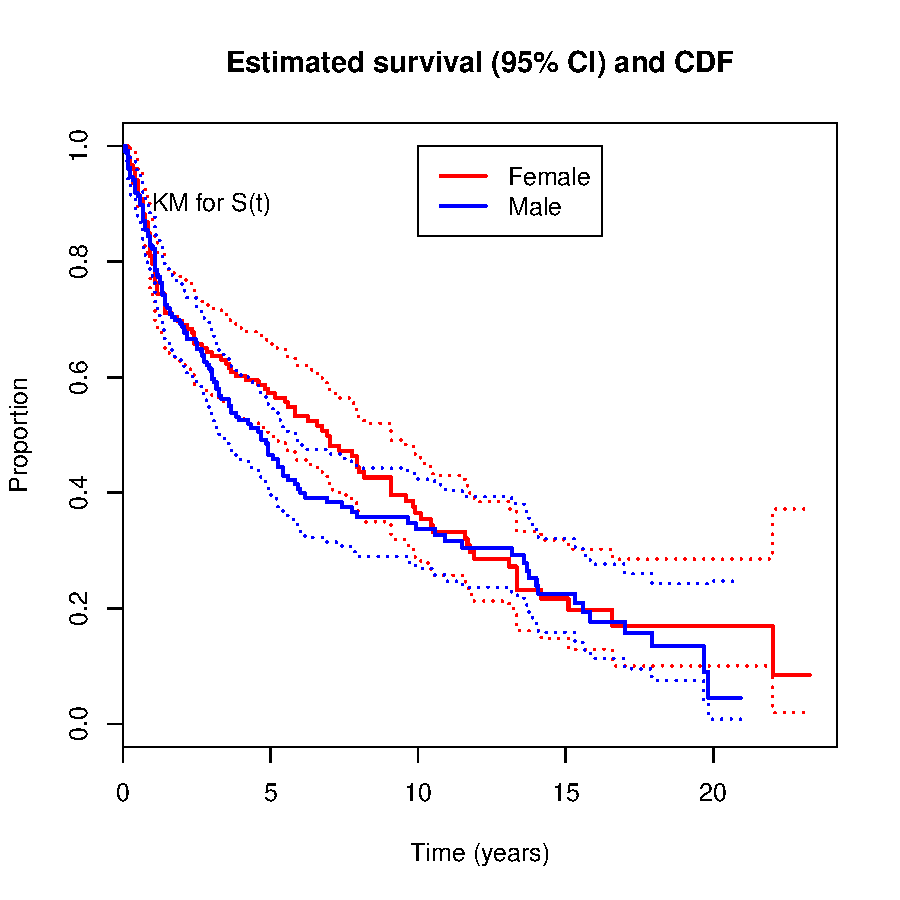
\includegraphics{Survival_competing_risk-km}


%\begin{figure}
%\centering
%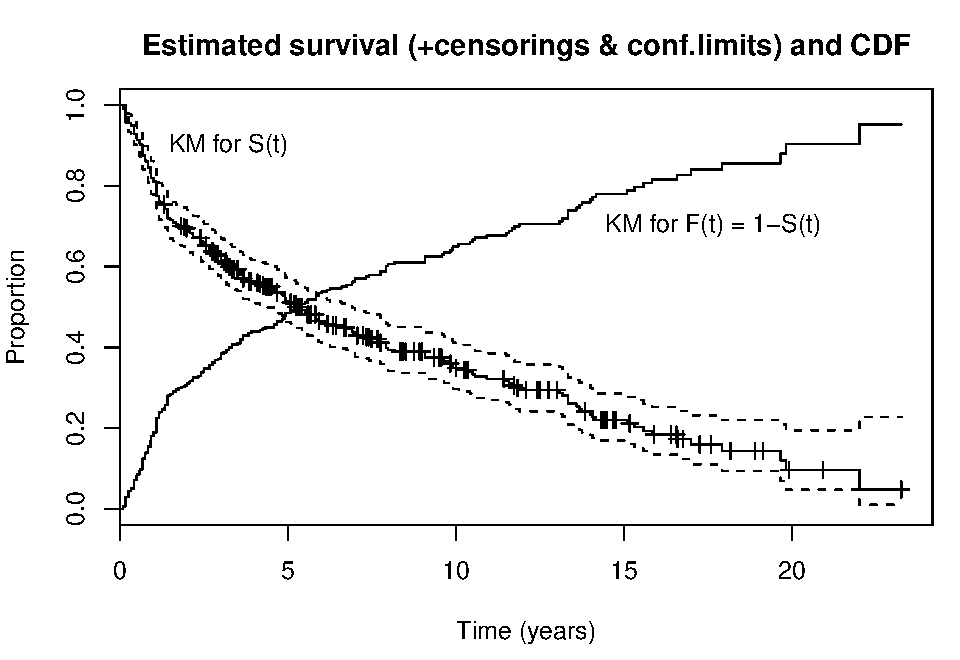
\includegraphics[width=1.0\textwidth]{orcaKM1} 
%\end{figure}

\end{frame}


\begin{frame}[fragile]
   \frametitle{Competing risks model: causes of death}
   
\begin{itemize}
\item
Often the interest is focused on the risk or hazard of dying 
from one specific cause.
\medskip
\item
That cause may eventually not be realized, because
a \textbf{competing cause} of death hits first.

\bigskip

\begin{center}
\setlength{\unitlength}{0.65pt}
\begin{picture}(400,190)
  \thicklines
  \put(  0, 115){\makebox(120,50)[b]{\footnotesize{(lex.Cst = 0)}}}
  \put(  0, 80){\framebox(130,60){Alive}}
  \put(  0, 80){\makebox(120,50)[b]{\footnotesize{(lex.Xst = 0)}}}
  %
  \put(230,130){\framebox(180,50){Dead from cancer}}
  \put(230, 130){\makebox(120,40)[b]{\scriptsize{(lex.Xst = 1)}}}
  %  \put(170, 97){(Cause-specific hazards)}
  \put(230, 30){\framebox(180,50){Dead, other causes}}
  \put(135,125){\vector(3, 1){90}}
  \put(230, 30){\makebox(120,30)[b]{\scriptsize{(lex.Xst = 2)}}}
%  \put(295,155){\vector(0,-1){100}}
  \put(135, 85){\vector(3,-1){90}}
  \put(165,157){\makebox(0,0)[b]{$\lambda_1(t)$}}
  \put(165, 53){\makebox(0,0)[t]{$\lambda_2(t)$}}
% \put(285,105){\makebox(0,0)[t]{$\nu$}}
\end{picture}
\end{center}
\item
 Generalizes to several competing causes.
 \end{itemize}
% Illness-death model. Little boxes with arrows.\\
% (The mortality of lung cancer patients ($\nu$) not relevant here).
\end{frame}

\begin{frame}[fragile]
\frametitle{Competing events \& competing risks}

In many epidemiological and clinical contexts there are
competing events that may 
occur before the target event and remove the person from 
 the population at risk for the event, \textit{e.g.}

\begin{itemize}
\item \textit{target event}: occurrence of endometrial cancer,
 \textit{competing events}: hysterectomy or death.
\medskip
\item \textit{target event}: relapse of a disease \\
(ending the state of remission), \\
 \textit{competing event}: death while still in remission.
 
% \medskip
\item \textit{target event}: divorce, \\ 
 \textit{competing event}: death of either spouse.
 
\end{itemize}

\end{frame}

\begin{frame}[fragile]
\frametitle{Event-specific quantities}

\textbf{Cumulative incidence function} (CIF) or \\
 %\textbf{subdistribution function} for event $c$:
\[  F_c(t) = P(T \leq t \text{ and } C = c ), \quad c = 1,2,  \]
%{subdensity function} $f_c(t) = dF_c(t)/dt$ 

\medskip
From these one can recover
\begin{itemize}
\item
$F(t) = \sum_{c} F_c(t)$, CDF of event-free survival time $T$, \textit{i.e.} 
cumulative risk of any event by $t$.
\medskip
\item
$S(t) = 1 - F(t)$, \textbf{event-free survival function}, \textit{i.e.} probability of avoiding all events by $t$, but $S(t) \ne F_1(t)+F_2(t)$
\end{itemize}
\end{frame}


\begin{frame}[fragile]
\frametitle{Event-specific quantities (cont'd)}

\textbf{Event-} or \textbf{cause-specific hazard function}
\begin{align*}
 \lambda_c(t) & =  \underset{\Delta\to 0}{\lim} 
    \frac{P(t < T \le t+\Delta \text{ and } C = c \mid T > t)}{\Delta}  \\
        & =  \frac{f_c(t)}{1-F(t)}
\end{align*}
% \underset{\Delta\to 0}{\lim} \frac{F_c(t+\Delta) - F_c(t)}{S(t)}/\Delta

CIF   =  risk of event $c$ over risk period $[0,t]$ in the presence of competing risks, also obtained 
$$ F_c(t) = \int_0^t \lambda_c(v) S(v) dv, \quad c = 1,2, $$

More on the technical definitions of relevant quantities:
http://bendixcarstensen.com/AdvCoh/papers/fundamentals.pdf

\end{frame}

\begin{frame}[fragile]
\frametitle{Warning of ``net risk'' and ``cause-specific survival''}

\begin{itemize}                              
\item
The ``\textbf{\textit{net risk}}'' of outcome $c$ by time $t$, 
assuming hypothetical elimination of competing risks,
is often defined as
\begin{center}
$ F_1^*(t) = 1 - S_1^*(t) = 1- \exp\{ - \Lambda_1(t) \} \ne S(t) $
% =1 - \exp\left\{ - \int_0^t h_c(v) dv \right\},  $$
\end{center}
\medskip
\item
In clinical survival studies, function 
$S_1^*(t)$ is often called ``\textbf{\textit{cause-specific survival}}'',
%and estimated by KM, but treating competing deaths
%as censorings.
or ``\textbf{\textit{net survival}}''
\medskip
\item
Yet, these *-functions, $ F_1^*(t)$ and $S_1^*(t)$, lack proper probability interpretation when
 competing risks exist.
\medskip
\item
Hence, their use 
%and naive KM estimation 
should be viewed critically
(Andersen \& Keiding, \textit{Stat Med}, 2012)
\end{itemize}
\end{frame}

%\begin{frame}
%   \frametitle{Example: Risk of lung cancer by age $a$?}
% \vspace*{-1em}
% \[
% \ptxt{Lung cancer before age 75} \ne 1-\e^{-\Lambda(75)}
% \]
% does not take the possibility of death prior to lung cancer into
% account.

%\begin{itemize}
% \item 
%  Empirical \textbf{cumulative rate} 
% CR$(a) = \sum_{k < a} I_k \Delta_k$, i.e.
%  ageband-width ($\Delta_k$) weighted 
%  sum of empirical 
%  age-specific incidence rates $I_k$
%  up to a given age $a$ \\
%  = estimate of cumulative hazard $\Lambda_c(a)$.
%  \medskip
%  \item 
%  Nordcan \& Globocan give 
% ``\textbf{\textit{cumulative risk}}'' by 75 y of age, computed from 
% $1 - \exp\{-\text{CR}(75)\}$, as an estimate  of the probability of 
% getting cancer before age $75$ y, 
% assuming that death were avoided by that age. This is based on 
% deriving ``net risk'' from cumulative hazard:
% \begin{center} 
% $ F_1^*(a) = 1 - \exp\{ - \Lambda_c(a) \}. $
% \end{center}
% \medskip
% \item
% Yet, cancer occurs in a mortal population.
% \medskip
% \item
% As such CR$({75})$ is a sound age-standardized summary 
%  measure for comparing cancer incidence across populations 
%  based on a neutral standard population.
% \end{itemize}
% 
% \end{frame}

%\begin{frame}
%\frametitle{Example. Male lung cancer in Denmark}

%Event-specific hazards: $\lambda_1(a)$ (lung cancer) death $\lambda_2(a)$ by age estimated by age-spec. rates.

%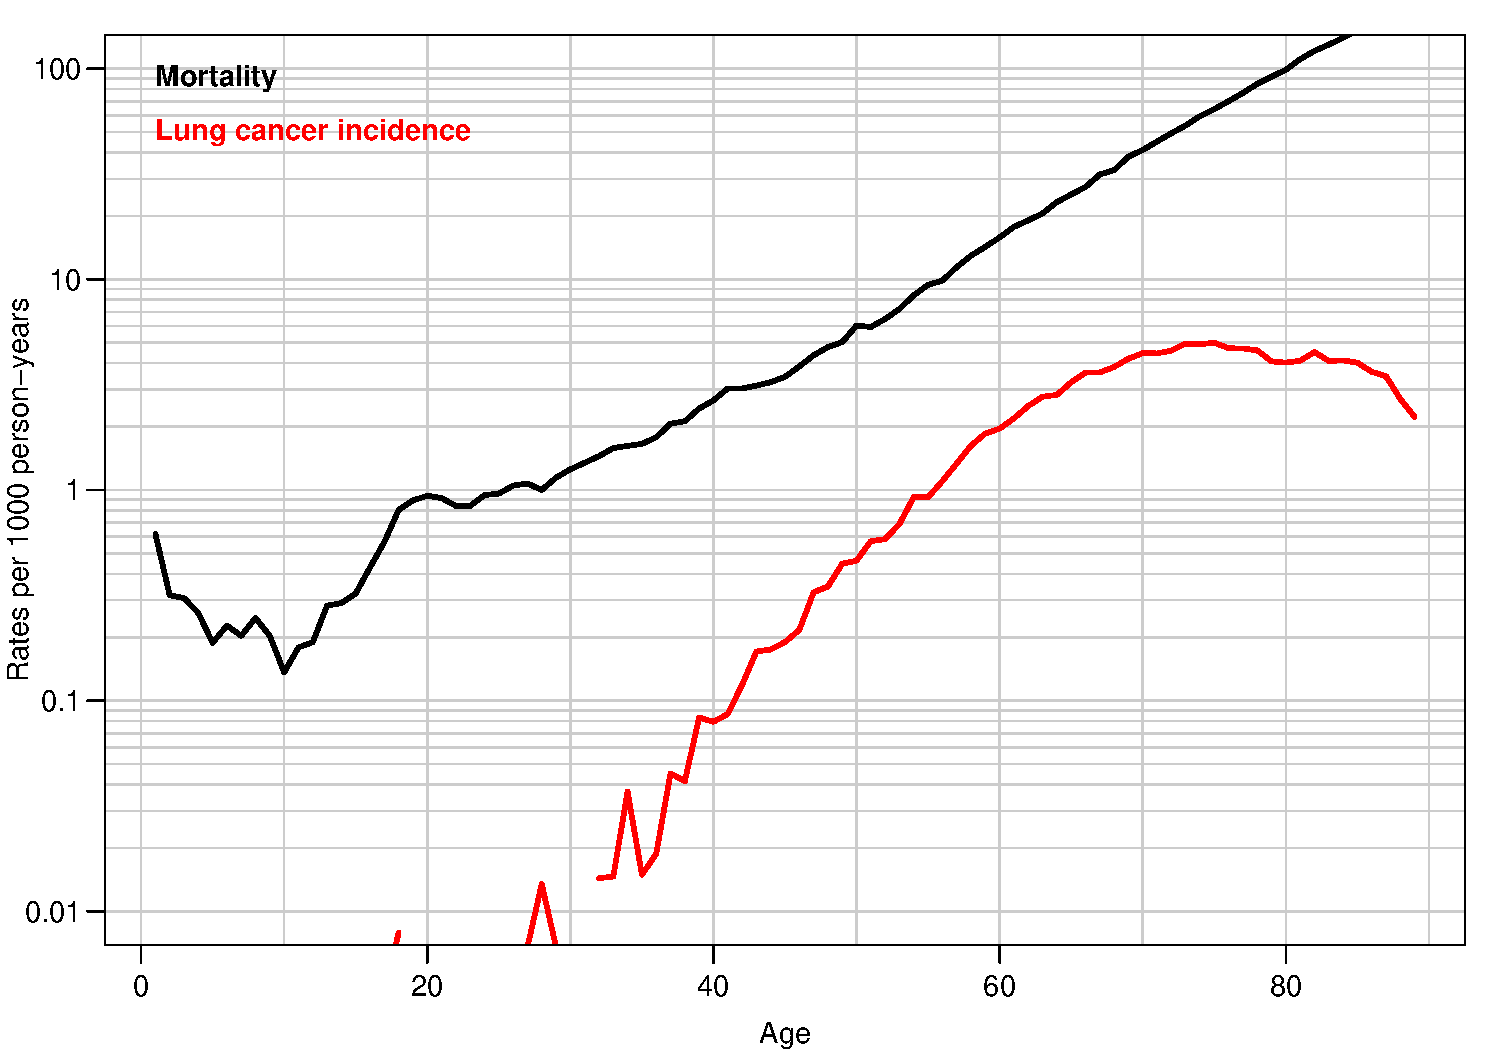
\includegraphics[height=6.5cm]{lung-ca-rates}
%\end{frame}

% \begin{frame}
% \frametitle{Cumulative incidence of lung cancer by age}
% 
% 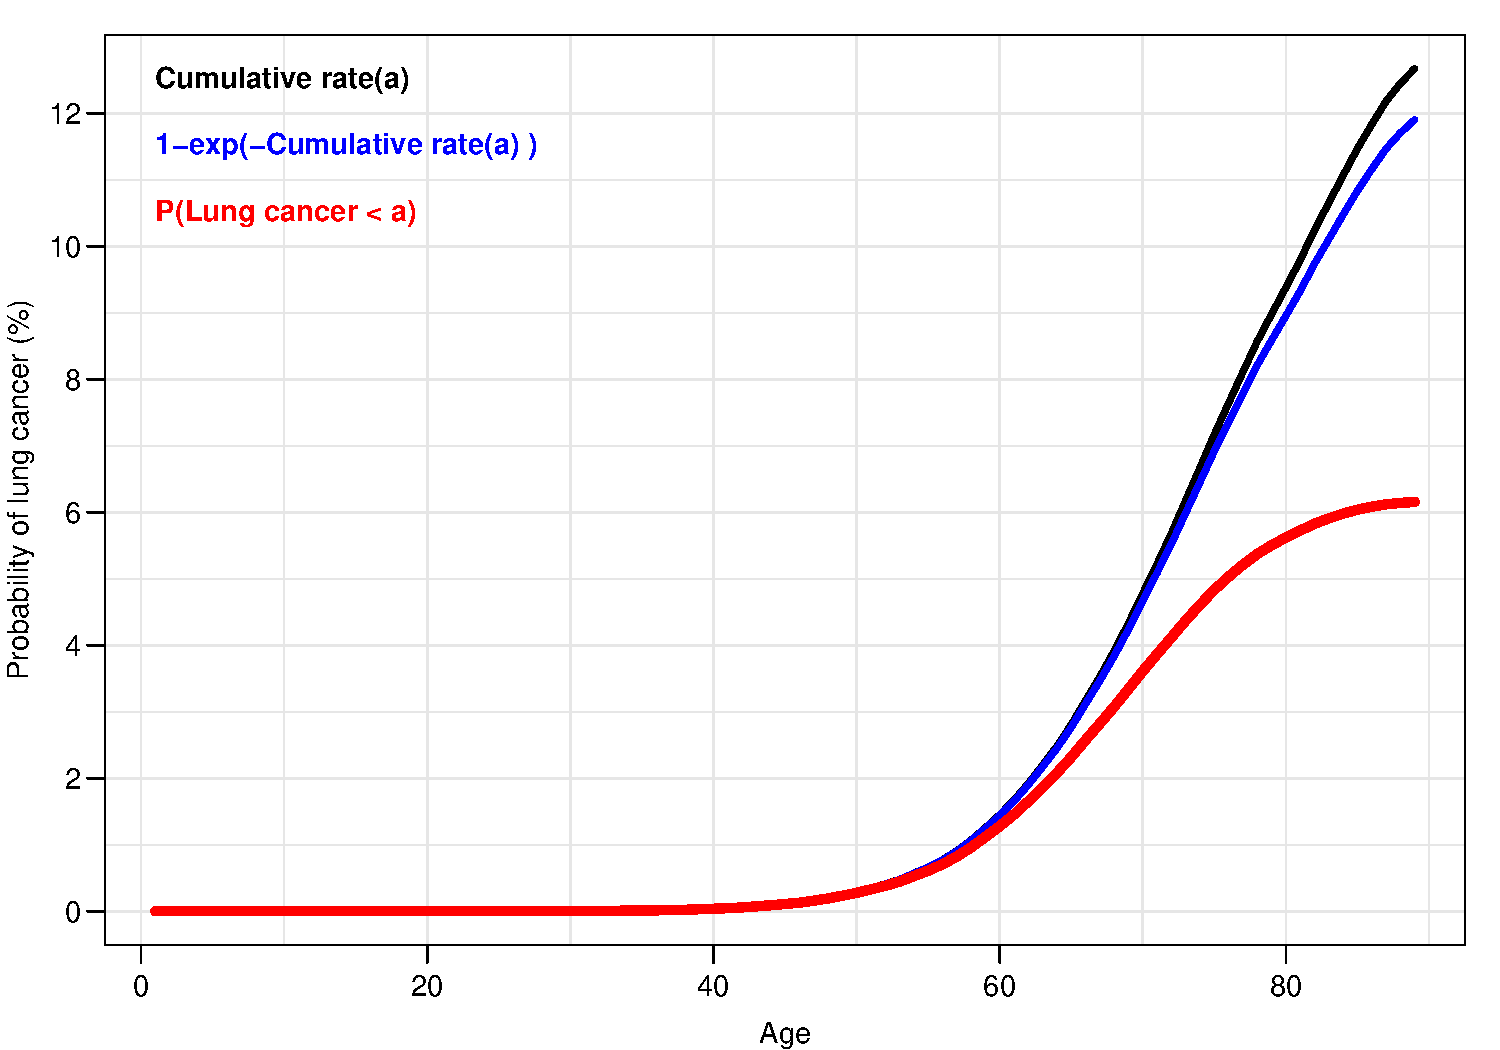
\includegraphics[height=6.5cm]{lung-ca-prob}
% 
% Both \text{CR} and $1 - \exp(- \text{CR})$ tend to \\
%  overestimate the real cumulative incidence CI after 60 y.
% \end{frame}


\begin{frame}[fragile]
\frametitle{Analysis with competing events}

Let $U_i$ = censoring time, 
% $\quad B_i$ = time of entry to follow-up (often $B_i = 0$),  \\
$T_i$ = time to first event, and \\
$C_i$ = variable for event 1 or 2. %, $i=1, \dots, n$. \\
We observe 
\begin{itemize}
\item $y_i = \text{min}\{ T_i, U_i \}$, \textit{i.e.}
the exit time, and
\item
 $ \delta_{ic} = 1_{ \{ T_i < U_i \ \& \ C_i = c\} }$, 
  indicator (1/0) for \\ 
  event $c$ being first observed, $c=1,2$. 
\end{itemize}


Non-parametric estimation % $\widetilde{F}_c(t)$ 
of CIF

\begin{itemize}
\item
Let $t_1 < t_2 < \dots < t_K$ be the $K$ distinct 
time points at which any outcome event was observed, \\ Let also
 $\widetilde{S}(t)$ be KM estimator for overall $S(t)$. 
\medskip
\item
\textbf{Aalen-Johansen estimator} (AJ) for the cumulative incidence function $F(t)$
should be used 
%is obtained as$$ \widetilde{F}_c(t) 
%   = \sum_{t_k \leq t} \frac{D_{kc}}{n_k} \times \widetilde{S}(t_{k-1}),
%   \quad\text{where}
%$$
%$n_k$ = size of the risk set at $t_k$ $(k=1, \dots, K)$,
%\\
%$D_{kc}$ = no. of cases of event $c$ observed  at $t_k$.
%\medskip
%\item
% \medskip
%Naive KM estimator $\widetilde{F}^*_c(t)$ of ``net survival'' treats  
%competing events occuring first as censorings:  
%$$  \widetilde{F}^*_c(t) = 1 - \widetilde{S}^*_c(t)
%  = 1 - \prod_{t_k \leq t} \frac{n_k - D_{kc}}{n_k} $$
\end{itemize}

\end{frame}

\begin{frame}[fragile]

\frametitle{R tools for competing risks analysis}

\begin{itemize}
% \item Covers even more general multi-state set-ups.
%  \pause
%  \medskip
\item \texttt{survfit( Surv(...,type="mstate") )} in Survival-package 
  can be fitted for any transition of a multistate model and to obtain A-J estimates.
% \item \texttt{Cuminc(time, status, ...)}:  \\
%  AJ-estimates (and SEs) for each event type 
% from observed follow-up times and events
%  (\texttt{status}, value 0 indicating censoring)
%\end{itemize}
\vspace*{1.0cm}
\item Package \texttt{cmprsk} --
 \texttt{cuminc(ftime, fstatus, ...)} 
  computes CIF-estimates,  % in \texttt{mstate},
  and can be compared in more than two samples.
   \texttt{plot.cuminc()} plots them. 
\vspace*{1.0cm}
\item Package \texttt{Epi} -- \texttt{Lexis} tools for multistate analyses \newline
 Will be advertised by Bendix!
 \end{itemize}

\end{frame}

%\begin{frame}[fragile]
%\frametitle{Ex. Survival from oral cancer}
% \begin{itemize}
% \item
% Creating a {\tt Lexis} object with two outcome events and \\ 
% obtaining a summary of transitions
% \end{itemize}
% \small
% \begin{verbatim}
% > orca.lex <- Lexis(exit = list(stime = time), 
%            exit.status = factor(event, 
%     labels = c("Alive", "Oral ca. death", "Other death") ),
%                   data = orca)
% 
% > summary(orca.lex)  
% Transitions:
%      To
% From    Alive Oral ca. Other  Records:  Events: Risk time:  Persons:
%   Alive   109      122   107       338      229    1913.67       338
% \end{verbatim}
% \normalsize
% 
% \end{frame}



\begin{frame}[fragile]
\frametitle{Box diagram for transitions}


{\scriptsize 
\begin{Schunk}
\begin{Soutput}
NOTE: entry.status has been set to "Alive" for all.
NOTE: entry is assumed to be 0 on the stime timescale.
\end{Soutput}
\end{Schunk}
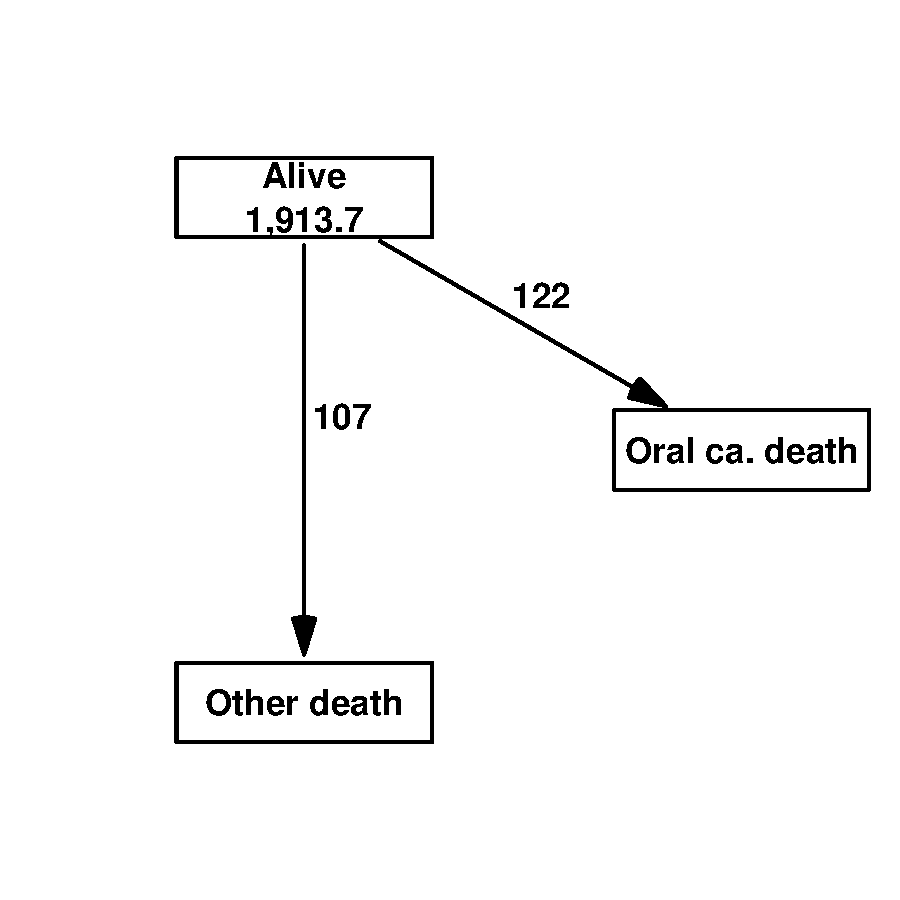
\includegraphics{Survival_competing_risk-boxplot}


}

\end{frame}

\begin{frame}[fragile]
\frametitle{Ex. Survival from oral cancer}
\begin{itemize}
\item
AJ-estimates of CIFs (solid) for both causes.
\item
Naive KM-estimates of CIF (dashed) $>$ AJ-estimates 
\item
CIF curves may also be stacked (right).  

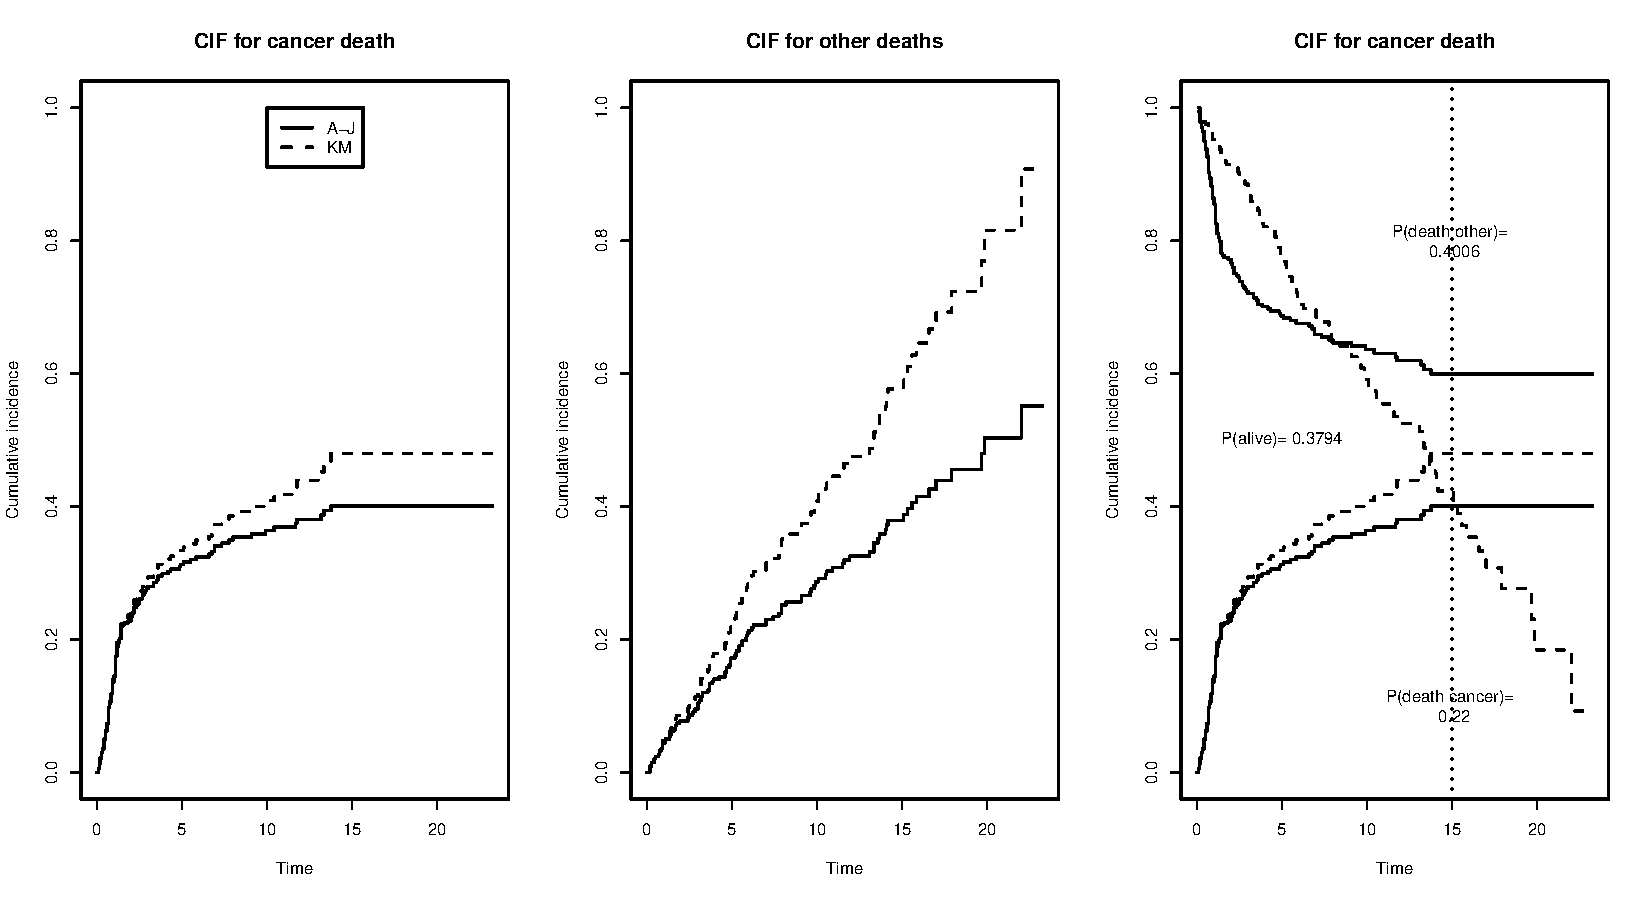
\includegraphics{Survival_competing_risk-plotcif1}

\end{itemize}


\textbf{NB.} The sum of the naive KM-estimates of CIF exceeds 100\% at 13 years! 
\end{frame}

\begin{frame}[fragile]
\frametitle{Ex. CIFs by cause in men and women}

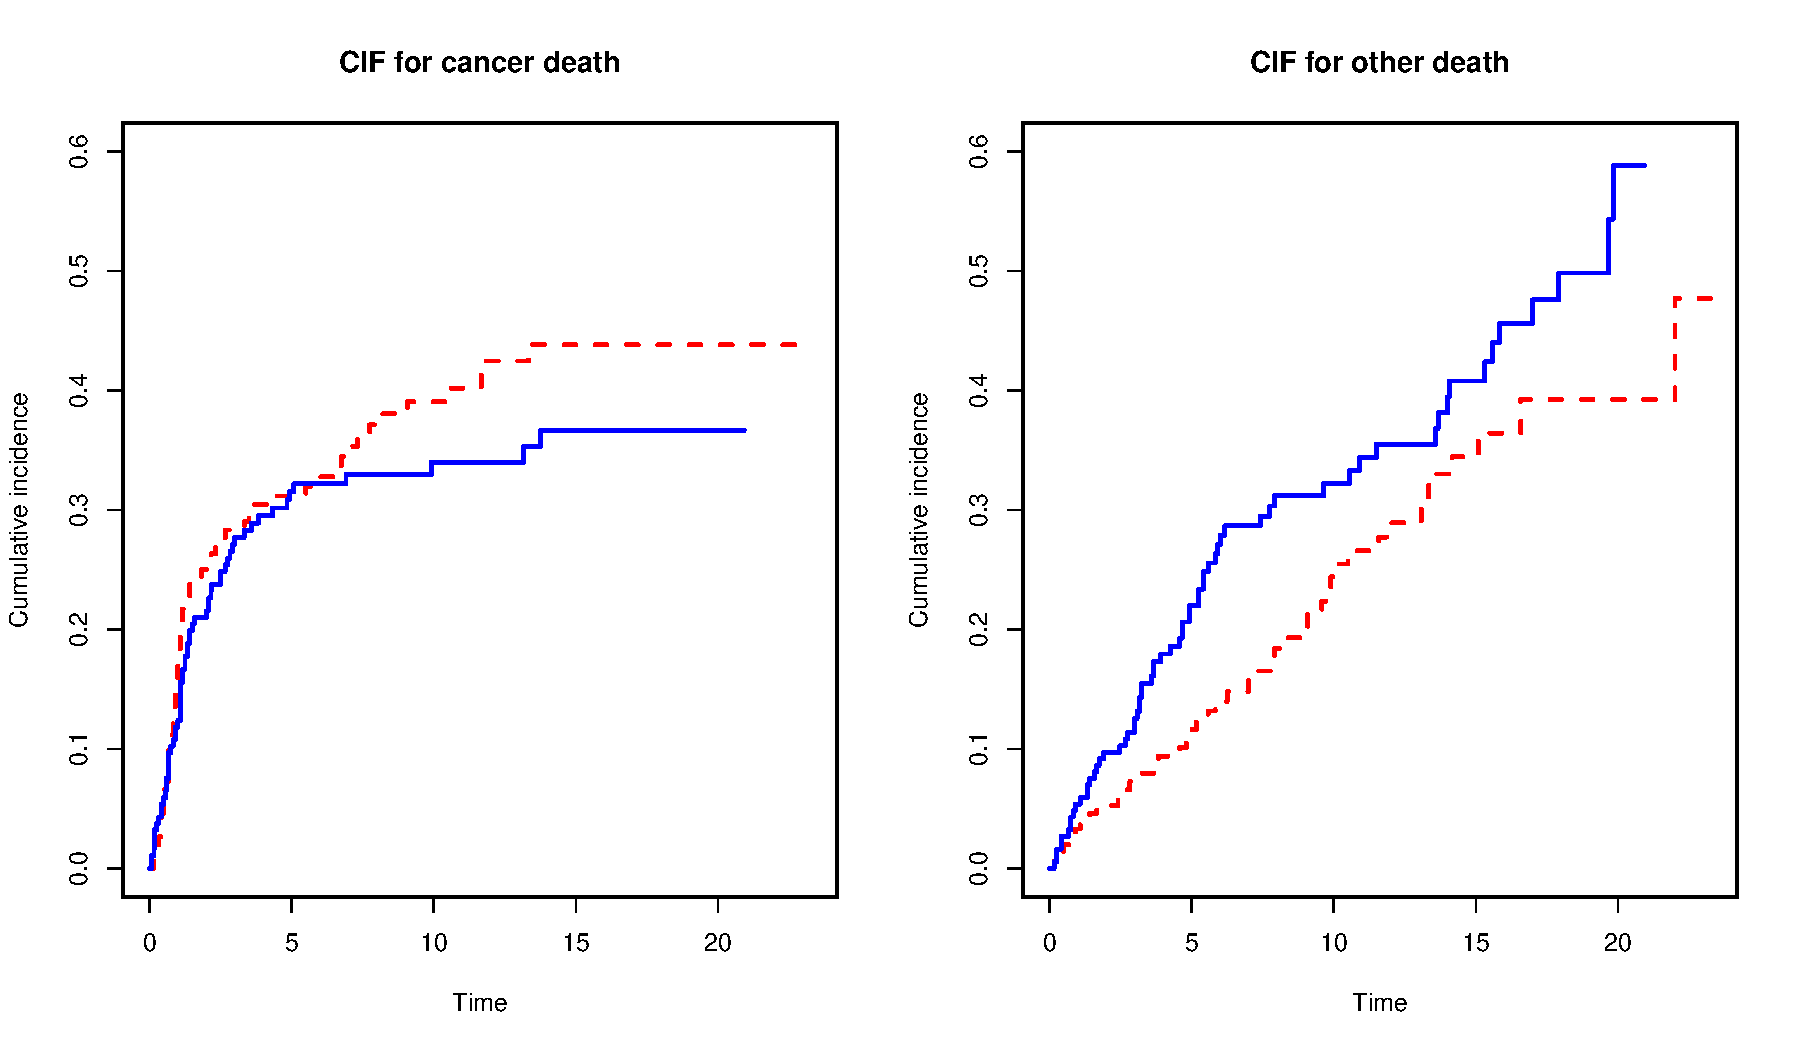
\includegraphics{Survival_competing_risk-plotcif2}

CIF for cancer higher in women (chance?) but for other causes
higher in men (no surprise).

\end{frame}

\begin{frame}[fragile]
\frametitle{Regression models for time-to-event data}


Regression models for hazards can be defined \textit{e.g.} for 
\begin{itemize}
% \item[(a)] survival times directly 
% $$ \log(T_i) = \eta_i + \epsilon_i, \quad\text{s.t. } 
% \epsilon_i \sim F_0(t; \alpha)$$ 
% where $F_0(t; \alpha)$ is some baseline model, 
% \medskip
% \pause
\item[(a)] hazards, multiplicatively: $$ 
\lambda_i(t) = \lambda_0(t; \alpha) r(\eta_i), \quad\text{where}$$
$\lambda_0(t; \alpha)$ = baseline hazard and \\
$r(\eta_i)$ = relative rate function, typically $\exp(\eta_i)$
\medskip
\pause
\item[(b)] hazards, additively: 
$$ \lambda_i(t) = \lambda_0(t; \alpha) + \eta_i. $$
\end{itemize}
\end{frame}


\begin{frame}[fragile]
\frametitle{Relative hazards model or Cox model}

In model (b), the baseline hazard $\lambda_0(t,\alpha)$ may be given a parametric form (\textit{e.g.} Weibull) or
a piecewise constant rate (exponential) structure.

\bigskip
Often a parameter-free form $\lambda_0(t)$ is assumed. Then
\[
  \lambda_i(t) = \lambda_0(t) \exp(\eta_1),
\]
specifies the \textbf{Cox model} or the \textbf{semiparametric proportional hazards model}.

\bigskip
$\eta_i = \beta_1 x_{i1} + \dots + \beta_p x_{ip}$ not depending on time.  

\bigskip
Generalizations: \textbf{time-dependent} \\ covariates $x_{ij}(t)$

% For exponential model, $\lambda_0(t) = \lambda_0$.

% Piecewise exponential model $\to$ constant baseline
% hazard in successive intervals:   
% \[ 
% \lambda_0(t) = \lambda_{0k}, \mbox{ for } 
% a_{k-1}} < t \leq a_k, \quad k = 1, 2, \dots, K 
% \]

\end{frame}


\begin{frame}[fragile]
\frametitle{PH model: interpretation of parameters}

Present the model explicitly in terms of $x$'s and $\beta$'s.
\[
\lambda_i(t) = \lambda_0(t)  \exp({\beta_1 x_{i1} + \dots +
\beta_p x_{ip}})
\]
Consider two individuals, $i$ and $i'$, having the same values of all
other covariates except the $j^{\text{th}}$ one.

\bigskip
The ratio of hazards is constant:
$$  \frac{\lambda_i(t)}{\lambda_{i'}(t)} = \frac{\exp( \eta_{i}) }{\exp(\eta_{i'})}
= \exp \{ \beta_j(x_{ij}-x_{i'j}) \} . $$
Thus $e^{\beta_j} = \text{HR}_j$ = \textbf{hazard ratio} or relative rate
 associated with
 a unit change in covariate $X_j$.

\end{frame}

\begin{frame}[fragile]
\frametitle{Ex. Total mortality of oral ca. patients}

Fitting Cox models with sex and sex + age.
\small
\begin{verbatim}
> cm0 <- coxph( suob ~ sex, data = orca)
> summary( cm0)
        coef exp(coef) se(coef)    z Pr(>|z|)
sexMale 0.126     1.134    0.134 0.94     0.35
        exp(coef) exp(-coef) lower .95 upper .95
sexMale      1.13      0.882     0.872      1.47

> cm1 <- coxph( suob ~ sex + age, data = orca)
> summary(cm1)
        exp(coef) exp(-coef) lower .95 upper .95
sexMale      1.49      0.669      1.14      1.96
age          1.04      0.960      1.03      1.05
\end{verbatim}
\normalsize
The M/F contrast visible only after age-adjustment.
\end{frame}

\begin{frame}[fragile]
\frametitle{Predictions from the Cox model}
\begin{itemize}
\item
Individual survival \textit{times} cannot be predicted
but ind'l survival \emph{curves} can.
PH model implies:
\[
S_i(t) = [S_0(t) ]^{\exp(\beta_1 x_{i1} +\ldots+\beta_p x_{ip})}
\]
\item
Having  estimated $\beta$ by partial likelihood, 
the baseline $S_0(t)$ is estimated by Breslow method 
\item 
\medskip
 From these, a survival curve for an individual
with given covariate values is predicted.
\item
\medskip
In R: 
\texttt{pred <- survfit(mod, newdata=...)} 
and \texttt{plot(pred)}, where \texttt{mod} is the fitted
\texttt{coxph} object, 
and \texttt{newdata}  
specifies the covariate values. \texttt{newdata} is always needed for
predictions.
\end{itemize}
\end{frame}

\begin{frame}[fragile]
\frametitle{Modelling with competing risks}

% When more than one outcome are operating,
% one may consider the 
Main options, providing answers to different questions.

\begin{itemize}
\item[(a)]
  Cox model for event-specific hazards $\lambda_c(t) = f_c(t)/[1-F(t)]$, when \textit{e.g.} the interest is in the biological effect of the prognostic factors on the fatality of the very disease that often leads to the relevant outcome.  
  \bigskip 
\item[(b)]
 \textbf{Fine--Gray model} for the hazard  of the subdistribution $\gamma_c(t) = f_c(t)/[1-F_c(t)]$ 
  when we want to assess the impact of the factors on the overall cumulative incidence of event $c$.  \\
  -- Function \texttt{crr()} in package \texttt{cmprsk}. 
\end{itemize}

\end{frame}

\begin{frame}[fragile]
   \frametitle{Competing risks model: excess hazard of death}


\begin{center}
\setlength{\unitlength}{0.65pt}
\begin{picture}(400,140)
  \thicklines
  \put(  0, 110){\framebox(120,50){Alive}}
  \put(115,0){\framebox(120,50){Dead}}
%  \put(170, 97){(Cause-specific hazards)}
  \put(230, 110){\framebox(120,50){Diseased}}
    \put(230, 110){\makebox(120,40)[b]{\scriptsize{($u = u_\text{D}$)}}}
  \put(125,105){\vector(1, -1){45}}
  \put(225,105){\vector(-1, -1){45}}
  \put(125, 135){\vector(1,0){100}}
  \put(170,137){\makebox(0,0)[b]{$\alpha(u)$}}
  \put(110, 95){\makebox(0,0)[t]{$\lambda_\text{P}(u)$}}
  \put(230, 90){\makebox(0,0)[t]{$\lambda(t)$}}
  %\put(315, 95){\makebox(0,0)[t]{$\lambda(t)=\lambda_1(t)+\lambda_2(t)$}}
  \put(350, 75){\makebox(0,0)[t]{$\lambda(t)=\lambda_\text{E}(t)+\lambda_\text{P}(u_\text{D}+t)$}}
  \put(300, 45){(excess mortality)}
  \put(350, 40){\makebox(0,0)[t]{$\lambda(t)= SMR \times \lambda_\text{P}(u_\text{D}+t)$}}
  \put(250, 10){(standardized mortality ratio)}
\end{picture}
\end{center}
where
\begin{itemize}
\item
 $\lambda_\text{P}(u)$ is the hazard of dying from any cause among disease-free members
 \item
   $\lambda_\text{E}(t)$ is the excess hazard of dying from the disease among diseased cohort members
 \end{itemize}

\end{frame}

\begin{frame}[fragile]
   \frametitle{Rectal cancer}

Ex. rectal cancers in females in Finland 2008-2012. Calculate observed mortality,
excess mortality and relative mortality.
{\footnotesize
\begin{Schunk}
\begin{Sinput}
> library(popEpi) # R-package for population-based cancer analysis- CRAN
> library(Epi)
> library(survival)
> data("sire")
> head(sire)
\end{Sinput}
\begin{Soutput}
   sex    bi_date    dg_date    ex_date status   dg_age
1:   1 1952-05-27 1994-02-03 2012-12-31      0 41.68877
2:   1 1959-04-04 1996-09-20 2012-12-31      0 37.46378
3:   1 1958-06-15 1994-05-30 2012-12-31      0 35.95616
4:   1 1957-05-10 1997-09-04 2012-12-31      0 40.32055
5:   1 1957-01-20 1996-09-24 2012-12-31      0 39.67745
6:   1 1962-05-25 1997-05-17 2012-12-31      0 34.97808
\end{Soutput}
\end{Schunk}
}
\end{frame}

\begin{frame}[fragile]
   \frametitle{Rectal cancer}

{\footnotesize
\begin{Schunk}
\begin{Sinput}
> data(sire)
>  ## split data
>  fotcut <- c(0,3/12,6/12,1,2,3,4,5)
>  lex.split <- lexpand(sire, birth = bi_date, entry = dg_date,
+                       exit = ex_date, 
+                       status=status %in% 1:2, 
+                       breaks = list(fot=fotcut), 
+                       pophaz=popmort,# population mortality
+                       pp=F, # weights for survival estimation
+                       aggre = list(fot) )
> head(lex.split)
\end{Sinput}
\begin{Soutput}
    fot     pyrs at.risk     d.exp from0to0 from0to1
1: 0.00 1946.997    8227  71.43614      105      717
2: 0.25 1779.831    7405  61.05649      103      431
3: 0.50 3215.778    6871 105.11004      190      633
4: 1.00 5459.795    6048 174.61314      340      791
5: 2.00 4501.971    4917 145.38757      294      492
6: 3.00 3825.438    4131 128.43103      281      322
\end{Soutput}
\end{Schunk}
}

\end{frame}


\begin{frame}[fragile]
   \frametitle{Rectal cancer -- mortality models}

Modeling mortality by splitted follow-up time since cancer diagnosis (fot)

Estimate excess mortality $\lambda_E(t)$ (link function d.exp)

{\scriptsize
\begin{Schunk}
\begin{Sinput}
> excess.mort <- relpois_ag(formula = from0to1 ~ -1 + fot,  
+ data = lex.split, 
+ d.exp = d.exp, 
+ offset = log(pyrs))
\end{Sinput}
\end{Schunk}
}

Estimate relative mortality (offset=log(d.exp))
{\scriptsize
\begin{Schunk}
\begin{Sinput}
> relative.mort <- glm(formula = from0to1 ~ -1 + as.factor(fot),
+ family=poisson(link="log"),
+ data=lex.split,
+ offset=log(d.exp))
\end{Sinput}
\end{Schunk}
}
Estimate observed mortality (offset=log(pyrs))
{\scriptsize
\begin{Schunk}
\begin{Sinput}
> obs.mort <- glm(formula = from0to1 ~ -1 + as.factor(fot),
+ family=poisson(link="log"),
+ data=lex.split,
+ offset=log(pyrs))
\end{Sinput}
\end{Schunk}
}


\end{frame}

\begin{frame}[fragile]
   \frametitle{Rectal cancer mortality}

Observed, expected, excess and relative mortality

{\footnotesize
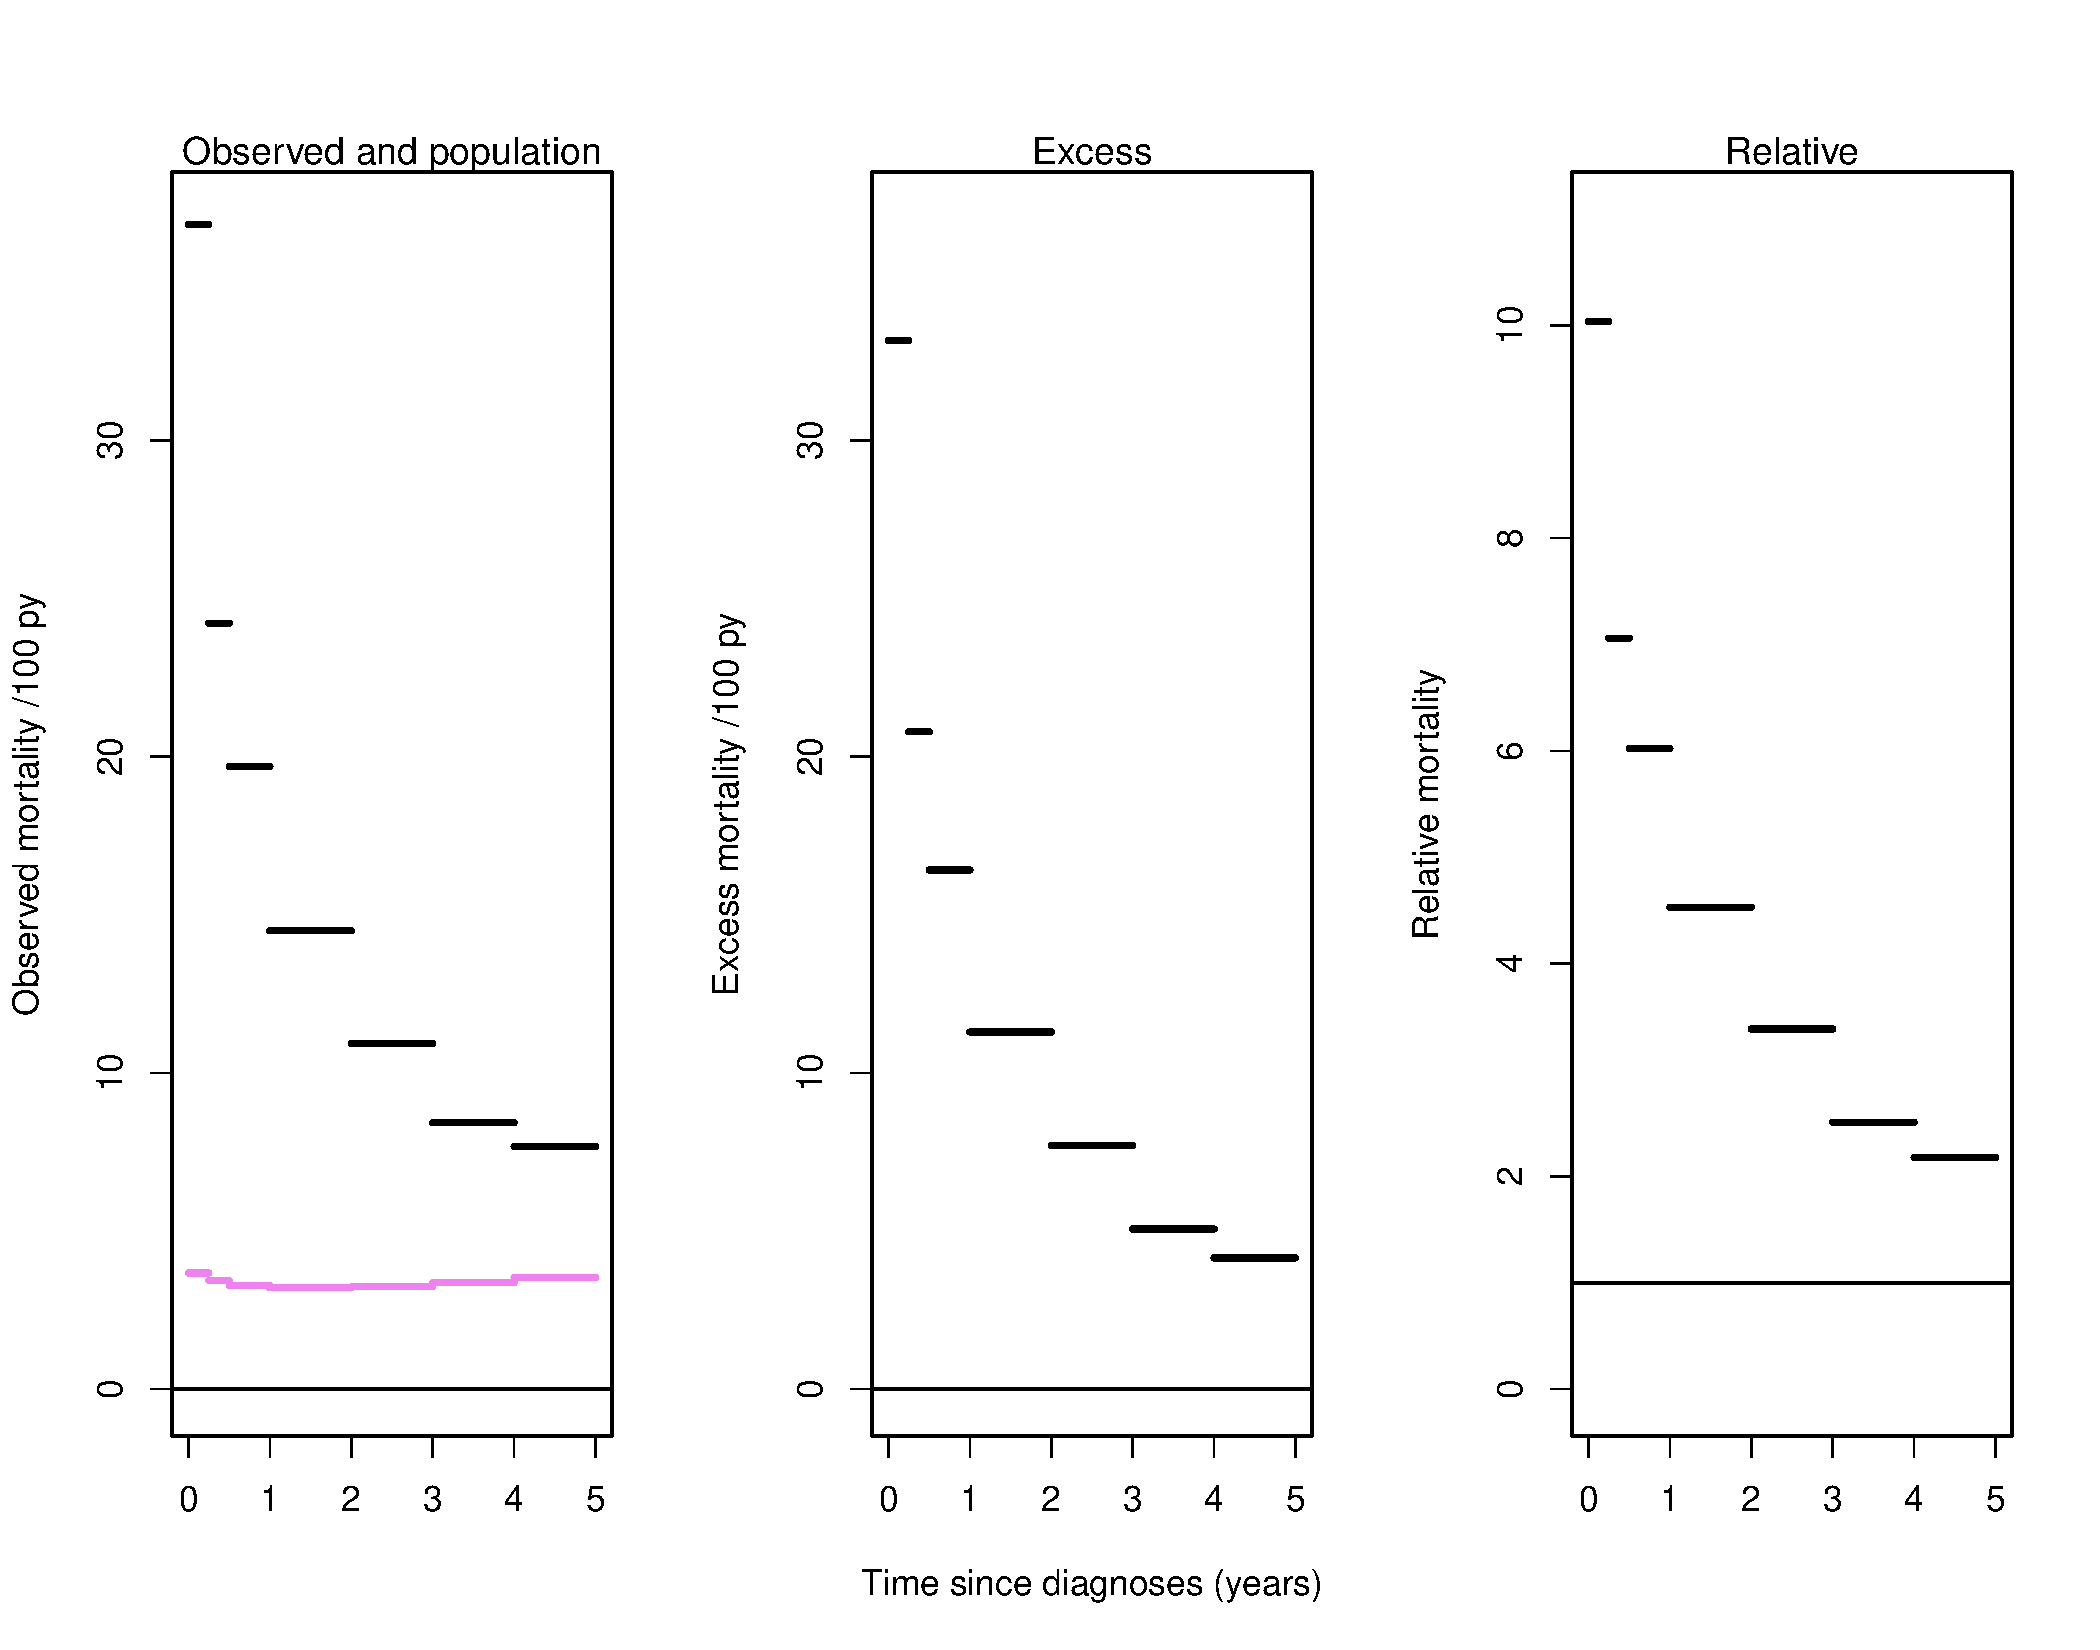
\includegraphics{Survival_competing_risk-em3}
}

\end{frame}

\end{document}
